\documentclass{article}

% If you're new to LaTeX, here's some short tutorials:
% https://www.overleaf.com/learn/latex/Learn_LaTeX_in_30_minutes
% https://en.wikibooks.org/wiki/LaTeX/Basics

% Formatting
\usepackage[utf8]{inputenc}
\usepackage[margin=1.5in]{geometry}
\usepackage[titletoc,title]{appendix}
% \usepackage{caption}
\usepackage{subcaption}
% Math
% https://www.overleaf.com/learn/latex/Mathematical_expressions
% https://en.wikibooks.org/wiki/LaTeX/Mathematics
\usepackage{amsmath,amsfonts,amssymb,mathtools}

% Images
% https://www.overleaf.com/learn/latex/Inserting_Images
% https://en.wikibooks.org/wiki/LaTeX/Floats,_Figures_and_Captions
\usepackage{graphicx,float}
\setlength{\parskip}{1.0em} 
% Tables
% https://www.overleaf.com/learn/latex/Tables
% https://en.wikibooks.org/wiki/LaTeX/Tables

% Algorithms
% https://www.overleaf.com/learn/latex/algorithms
% https://en.wikibooks.org/wiki/LaTeX/Algorithms
\usepackage[ruled,vlined]{algorithm2e}
\usepackage{algorithmic}

% Code syntax highlighting
% https://www.overleaf.com/learn/latex/Code_Highlighting_with_minted
\usepackage{minted}
\usemintedstyle{borland}

% References
% https://www.overleaf.com/learn/latex/Bibliography_management_in_LaTeX
% https://en.wikibooks.org/wiki/LaTeX/Bibliography_Management
\usepackage{biblatex}
\addbibresource{references.bib}

% Title content
\title{CS 529 Project 3}
\author{Connor Frost}
\date{May 3, 2020}

\begin{document}

\maketitle

% Introduction and Overview
\section*{Introduction}

The data used for training the classifier are tweets that are labeled either zero (for negative sentiment) and one (for positive sentiment). These tweets can be broken down and learned from using each individual word to learn the association between a word and its associated sentiment.

\section{Bayesian Classification for Tweet Sentiments}

There are three main parts for the classification:

\begin{itemize}
    \item Extraction and counting of vocab
    \item Training the model
    \item Prediction using the vocab and priors.
\end{itemize}

\noindent These are further elaborated upon and implemented within the code.

\subsection{Code}

Inspiration is taken from https://medium.datadriveninvestor.com/implementing-naive-bayes-for-sentiment-analysis-in-python-951fa8dcd928 which was posted by Zachary Clarke on the Piazza page. However, it has to be implemented for our data and uses some of the feature selection mentioned in the assignment. This feature selection is elaborated upon in the accuracy analysis. 

\noindent The model is trained on the training data, and then subsequently predicts the election data. The code for this training and election data prediction is attached as: naive\_bayes\_classifier.py

\subsection{Accuracy Benchmarks and Analysis}

The following graph shows the accuracy while training. Each epoch is a tweet that the vocab is learned from. 

\begin{figure}[h!]
    \centering
    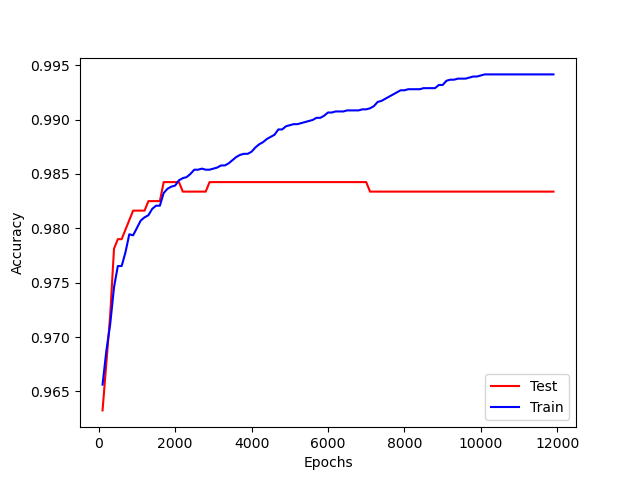
\includegraphics[width=1\linewidth]{plots/Epoch_Accuracy.png}
    \caption*{Accuracy vs Epoch. Where each epoch is a tweet to train off of.}
\end{figure}    

\noindent Using each tweet as an epoch can help describe the trend in training and testing. Doing this, we also learn that most of the training occurs very early (within the first 10 tweets to get 90\%+ accuracy), seemingly by relying on the emojis as part of the vocab. The accuracy is probably so high because of the use of the emojis which help indicate the sentiment (which may also be the way this data was collected). 

\noindent Some words are filtered out such as articles of the English language, urls, and the people who are tagged in posts. Some moderate boosts in accuracy were obtained by excluding these certain words as they may have initially confused the model. The accuracy boost was only around 0.5\%  from 97.8\% to 98.35\% on the test data by filtering out these words.  

\noindent This graph is produced by naive\_bayes\_classifier\_analysis.py

\section{Time Analysis of Election Tweets}

For the analysis of the sentiment for election tweets, the following is observed when separating the data into the following three categories
\begin{itemize}
    \item Before the election results started coming in, in order to get the average sentiment of people before the news of the election started trickling in. This was the night of November 3rd.
    \item During the election results reporting. This is important to distinguish because the election was called days later (most organizations called on November 7th but some on November 6th), and this may be important to distinguish from post-election sentiment
    \item After the election was called which helps capture people's sentiment when the projections were announced.
\end{itemize}

\noindent Using these distinctions and by organizing the predicted sentiments into each of the above categories, we can take the average of the predicted sentiments for tweets to be able to calulate the average sentiment expressed by people during these times. 

\noindent The following average sentiments are predicted for the above timeframes respectively: 

\begin{itemize}
    \item Before Election: 0.5763195435092725
    \item During Election: 0.49295774647887325
    \item After Election: 0.5156537753222836
\end{itemize}

\noindent While the sentiment is oftentimes hard to compute for each individual tweet given the multitude of complexities of people expressing their political ideologies, the calculated average sentiment seems to have been the lowest when the results were still being reported on. This may be caused from the anxiety that people may have experienced while not knowing for certain. The highest sentiment was expressed before the election which may be caused from the optimism that many people seem to have placed in their opponent. 

\noindent The analysis interestingly seems to capture the sway in emotions during the distinctive time frames. 

\noindent This analysis is found using the attached python program: election\_analysis.py

\section*{Files}

The following help describe the submitted files.

\begin{itemize}
    \item readme.md for getting started with the python files.
    \item *.py files for analysis and training. (Further elaborated within the document
    \item ./data/ directory that the python files use to read datasets and save predictions
\end{itemize}

\end{document}

